\subsection{Model 2: Transformer}
The model is made from the solution to exercise sheet 5. Very few elements have been changed since it follows the pages in the Bishop book closely. The only big changes that has been made to the model itself is added dropout layers and positional encoding. We also experimented with randomly removing 2 tokens from each sentence to increase generalisation but it didn't work. WE also tried adding 2 more linear layers to the transformer block, but this was detrimental to the accuracy so we removed them again.
We chose to use a transformer model as it seems like a good architecture for working with text since it makes words weigh differently depending on which other words are present in the sentence, and with positional encoding also where they are in that sentence. This is important since the meaning of words change depending on other words, and position in sentence.
We used sinusoidal position embedding since this is the positional embedding used in the Bishop book.
The L in the sinusoidal position embedding is 10000. The example in the Bishop book had an L of 30, and some other examples we encountered had an L of 10000. We chose 10000 as the value for L since we encountered it multiple places.\\

We used cross entropy loss as a our loss function since this is a good loss function for classification tasks.
This is the number of heads in the multi head self attention mechanism. d\_model should preferably be divisible by this number so each head computes the same size of input. We chose 8 heads since having too many heads can be inefficient and since we have d\_model of 128, choosing more heads would lead to quite few dimensions per head, which would make it hard for them to capture any useful features.
The mlp factor controls the amount of nodes in the linear layers of the transformer block. We use an mlp factor of 4. This was the default value and decreasing this value hit the performance of the model. Increasing the mlp factor would increase the training time so we decided to not do that.
d\_model is the dimensions of each token. We have a vocabulary of 10336 so we made this pretty big to ensure that each word is able to be uniquely represented. \\

We have 6 layers of transformer blocks. According to the slides, 6 layers is a normal amount of layers and 12 layers is for very large models. We experimented with 6 and 12 layers and found only a small performance increase with 12 layers, but a significant increase in training time, so we decided that we would rather train quicker to test values for other parameters.
When training the transformer models with different parameters we found out that they would quickly overfit, so we needed to generalise the model. To do this we added two dropout layers on the linear layers of the transformer blocks. The dropout chance for the first layer is 50\% and for the second layer is 25\%. We tested with both higher and lower dropout chances and this worked the best.
We chose adam as the optimizer. From the last project our and other peoples takeaway were that adam was a good optimizer in general, and since were not using weight decay, we don't need to use adamW.
We used a learning rate of 0,0003. This was discussed as a good learning rate from the last project, and our experimenting also led us to this learning rate.
We experimented a bit with using weight decay but it did not work well so we decided not to use it in our final model.
When testing different parameters, we used 50 epochs. The transformer models quickly overfitted so we didn't need more epochs. 
We experimented with both L1 and L2 regularisation. L1 regularisation worked the best, and that is probably because it makes some weights go to 0, which indicates those words aren't important. In sentences, some words tells more than other words, so it makes sense that this would be good.

\begin{figure}[H]
    \vspace*{0.7cm}
    \centering
    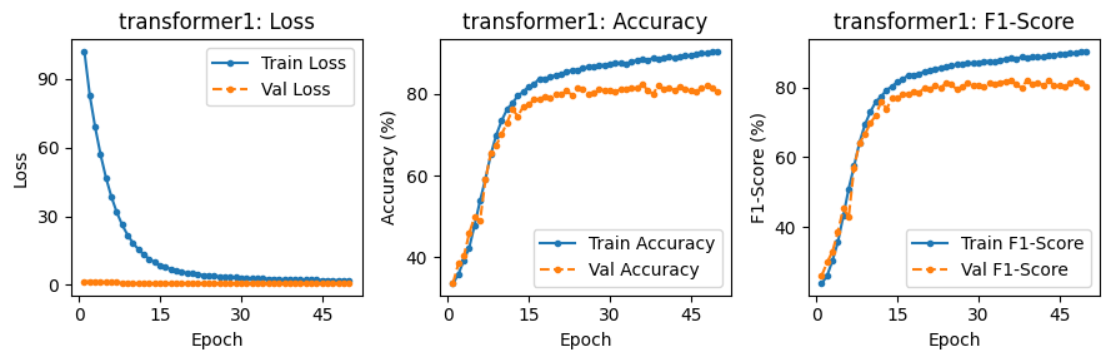
\includegraphics[width=0.6\textwidth]{figures/transformer_scores.png}
    \caption{Training and validation loss, accuracy, and F1-score for the transformer model.}
    \label{fig:transformer_scores}
    \vspace*{0.7cm}
\end{figure}

\begin{table}[H]
    \vspace*{-0.5cm}
    \centering
    \begin{tabular}{|l|c|c|c|}
        \hline
        Label        & Precision & Recall & F1-Score \\ \hline
        sadness      & 0.89      & 0.82   & 0.85     \\ \hline
        joy          & 0.81      & 0.88   & 0.85     \\ \hline
        love         & 0.68      & 0.59   & 0.63     \\ \hline
        anger        & 0.77      & 0.81   & 0.79     \\ \hline
        fear         & 0.80      & 0.80   & 0.80     \\ \hline
        surprise     & 0.67      & 0.56   & 0.61     \\ \hline\hline
        accuracy     &           &        & 0.81     \\ \hline
        weighted avg & 0.81      & 0.81   & 0.81     \\ \hline
    \end{tabular}
    \caption{Transformer model performance on test set.}
    \label{tab:rnn_lstm_model_test}
    \vspace*{-0.8cm}
\end{table}

Despite a lot of parameter tuning, we could not get the transformer model to get a better performance. We even tried adding extra linear layers in the transformer block, and removing random words from the sentences for better generalisation.
